\documentclass[11pt]{article}

    %\usepackage[breakable]{tcolorbox}
    \usepackage[most]{tcolorbox}
    \usepackage{lmodern} 
    \usepackage{parskip} % Stop auto-indenting (to mimic markdown behaviour)
    
    \usepackage{iftex}
    \ifPDFTeX
    	\usepackage[T1]{fontenc}
    	\usepackage{mathpazo}
    \else
    	\usepackage{fontspec}
    \fi

    % Basic figure setup, for now with no caption control since it's done
    % automatically by Pandoc (which extracts ![](path) syntax from Markdown).
    \usepackage{graphicx}
    % Maintain compatibility with old templates. Remove in nbconvert 6.0
    \let\Oldincludegraphics\includegraphics
    % Ensure that by default, figures have no caption (until we provide a
    % proper Figure object with a Caption API and a way to capture that
    % in the conversion process - todo).
    \usepackage{caption}
    \DeclareCaptionFormat{nocaption}{}
    \captionsetup{format=nocaption,aboveskip=0pt,belowskip=0pt}

    \usepackage{float}
    \floatplacement{figure}{H} % forces figures to be placed at the correct location
    \usepackage{xcolor} % Allow colors to be defined
    \usepackage{enumerate} % Needed for markdown enumerations to work
    \usepackage{geometry} % Used to adjust the document margins
    \usepackage{amsmath} % Equations
    \usepackage{amssymb} % Equations
    \usepackage{textcomp} % defines textquotesingle
    % Hack from http://tex.stackexchange.com/a/47451/13684:
    \AtBeginDocument{%
        \def\PYZsq{\textquotesingle}% Upright quotes in Pygmentized code
    }
    \usepackage{upquote} % Upright quotes for verbatim code
    \usepackage{eurosym} % defines \euro
    \usepackage[mathletters]{ucs} % Extended unicode (utf-8) support
    \usepackage{fancyvrb} % verbatim replacement that allows latex
    \usepackage{grffile} % extends the file name processing of package graphics 
                         % to support a larger range
    \makeatletter % fix for old versions of grffile with XeLaTeX
    \@ifpackagelater{grffile}{2019/11/01}
    {
      % Do nothing on new versions
    }
    {
      \def\Gread@@xetex#1{%
        \IfFileExists{"\Gin@base".bb}%
        {\Gread@eps{\Gin@base.bb}}%
        {\Gread@@xetex@aux#1}%
      }
    }
    \makeatother
    \usepackage[Export]{adjustbox} % Used to constrain images to a maximum size
    \adjustboxset{max size={0.9\linewidth}{0.9\paperheight}}

    % The hyperref package gives us a pdf with properly built
    % internal navigation ('pdf bookmarks' for the table of contents,
    % internal cross-reference links, web links for URLs, etc.)
    \usepackage{hyperref}
    % The default LaTeX title has an obnoxious amount of whitespace. By default,
    % titling removes some of it. It also provides customization options.
    \usepackage{titling}
    \usepackage{longtable} % longtable support required by pandoc >1.10
    \usepackage{booktabs}  % table support for pandoc > 1.12.2
    \usepackage[inline]{enumitem} % IRkernel/repr support (it uses the enumerate* environment)
    \usepackage[normalem]{ulem} % ulem is needed to support strikethroughs (\sout)
                                % normalem makes italics be italics, not underlines
    \usepackage{mathrsfs}
    
\usepackage{fancyhdr}
\usepackage{lastpage}
\usepackage{cclicenses}

    % Colors for the hyperref package
    \definecolor{urlcolor}{rgb}{0,.145,.698}
    \definecolor{linkcolor}{rgb}{.71,0.21,0.01}
    \definecolor{citecolor}{rgb}{.12,.54,.11}

    % ANSI colors
    \definecolor{ansi-black}{HTML}{3E424D}
    \definecolor{ansi-black-intense}{HTML}{282C36}
    \definecolor{ansi-red}{HTML}{E75C58}
    \definecolor{ansi-red-intense}{HTML}{B22B31}
    \definecolor{ansi-green}{HTML}{00A250}
    \definecolor{ansi-green-intense}{HTML}{007427}
    \definecolor{ansi-yellow}{HTML}{DDB62B}
    \definecolor{ansi-yellow-intense}{HTML}{B27D12}
    \definecolor{ansi-blue}{HTML}{208FFB}
    \definecolor{ansi-blue-intense}{HTML}{0065CA}
    \definecolor{ansi-magenta}{HTML}{D160C4}
    \definecolor{ansi-magenta-intense}{HTML}{A03196}
    \definecolor{ansi-cyan}{HTML}{60C6C8}
    \definecolor{ansi-cyan-intense}{HTML}{258F8F}
    \definecolor{ansi-white}{HTML}{C5C1B4}
    \definecolor{ansi-white-intense}{HTML}{A1A6B2}
    \definecolor{ansi-default-inverse-fg}{HTML}{FFFFFF}
    \definecolor{ansi-default-inverse-bg}{HTML}{000000}

    % common color for the border for error outputs.
    \definecolor{outerrorbackground}{HTML}{FFDFDF}

    % commands and environments needed by pandoc snippets
    % extracted from the output of `pandoc -s`
    \providecommand{\tightlist}{%
      \setlength{\itemsep}{0pt}\setlength{\parskip}{0pt}}
    \DefineVerbatimEnvironment{Highlighting}{Verbatim}{commandchars=\\\{\}}
    % Add ',fontsize=\small' for more characters per line
    \newenvironment{Shaded}{}{}
    \newcommand{\KeywordTok}[1]{\textcolor[rgb]{0.00,0.44,0.13}{\textbf{{#1}}}}
    \newcommand{\DataTypeTok}[1]{\textcolor[rgb]{0.56,0.13,0.00}{{#1}}}
    \newcommand{\DecValTok}[1]{\textcolor[rgb]{0.25,0.63,0.44}{{#1}}}
    \newcommand{\BaseNTok}[1]{\textcolor[rgb]{0.25,0.63,0.44}{{#1}}}
    \newcommand{\FloatTok}[1]{\textcolor[rgb]{0.25,0.63,0.44}{{#1}}}
    \newcommand{\CharTok}[1]{\textcolor[rgb]{0.25,0.44,0.63}{{#1}}}
    \newcommand{\StringTok}[1]{\textcolor[rgb]{0.25,0.44,0.63}{{#1}}}
    \newcommand{\CommentTok}[1]{\textcolor[rgb]{0.38,0.63,0.69}{\textit{{#1}}}}
    \newcommand{\OtherTok}[1]{\textcolor[rgb]{0.00,0.44,0.13}{{#1}}}
    \newcommand{\AlertTok}[1]{\textcolor[rgb]{1.00,0.00,0.00}{\textbf{{#1}}}}
    \newcommand{\FunctionTok}[1]{\textcolor[rgb]{0.02,0.16,0.49}{{#1}}}
    \newcommand{\RegionMarkerTok}[1]{{#1}}
    \newcommand{\ErrorTok}[1]{\textcolor[rgb]{1.00,0.00,0.00}{\textbf{{#1}}}}
    \newcommand{\NormalTok}[1]{{#1}}
    
    % Additional commands for more recent versions of Pandoc
    \newcommand{\ConstantTok}[1]{\textcolor[rgb]{0.53,0.00,0.00}{{#1}}}
    \newcommand{\SpecialCharTok}[1]{\textcolor[rgb]{0.25,0.44,0.63}{{#1}}}
    \newcommand{\VerbatimStringTok}[1]{\textcolor[rgb]{0.25,0.44,0.63}{{#1}}}
    \newcommand{\SpecialStringTok}[1]{\textcolor[rgb]{0.73,0.40,0.53}{{#1}}}
    \newcommand{\ImportTok}[1]{{#1}}
    \newcommand{\DocumentationTok}[1]{\textcolor[rgb]{0.73,0.13,0.13}{\textit{{#1}}}}
    \newcommand{\AnnotationTok}[1]{\textcolor[rgb]{0.38,0.63,0.69}{\textbf{\textit{{#1}}}}}
    \newcommand{\CommentVarTok}[1]{\textcolor[rgb]{0.38,0.63,0.69}{\textbf{\textit{{#1}}}}}
    \newcommand{\VariableTok}[1]{\textcolor[rgb]{0.10,0.09,0.49}{{#1}}}
    \newcommand{\ControlFlowTok}[1]{\textcolor[rgb]{0.00,0.44,0.13}{\textbf{{#1}}}}
    \newcommand{\OperatorTok}[1]{\textcolor[rgb]{0.40,0.40,0.40}{{#1}}}
    \newcommand{\BuiltInTok}[1]{{#1}}
    \newcommand{\ExtensionTok}[1]{{#1}}
    \newcommand{\PreprocessorTok}[1]{\textcolor[rgb]{0.74,0.48,0.00}{{#1}}}
    \newcommand{\AttributeTok}[1]{\textcolor[rgb]{0.49,0.56,0.16}{{#1}}}
    \newcommand{\InformationTok}[1]{\textcolor[rgb]{0.38,0.63,0.69}{\textbf{\textit{{#1}}}}}
    \newcommand{\WarningTok}[1]{\textcolor[rgb]{0.38,0.63,0.69}{\textbf{\textit{{#1}}}}}
    
    % Slightly bigger margins than the latex defaults
    
    \geometry{verbose,tmargin=0.7in,bmargin=0.7in,lmargin=0.7in,rmargin=0.7in}
        
    % Define a nice break command that doesn't care if a line doesn't already
    % exist.
    \def\br{\hspace*{\fill} \\* }
    % Math Jax compatibility definitions
    \def\gt{>}
    \def\lt{<}
    \let\Oldtex\TeX
    \let\Oldlatex\LaTeX
    \renewcommand{\TeX}{\textrm{\Oldtex}}
    \renewcommand{\LaTeX}{\textrm{\Oldlatex}}
    % Document parameters
    % Document title
    \title{Opérateurs logiques}
      \date{Octobre 2021}  
	%\author{Yannick Chistel}
    
\makeatletter         
\renewcommand\maketitle[1]{
\hrule\medskip
{\raggedright % Note the extra {
\begin{center}
{\Huge \bfseries \sffamily #1 }\\[4ex] 
%{\Large  \@author}\\[2ex] 
%\@date\\[4ex]
\hrule \bigskip
\end{center}}} % Note the extra }
\makeatother    



\pagestyle{fancy}
\fancyhead{}
\renewcommand\headrulewidth{0pt}
\renewcommand\footrulewidth{1pt}
\fancyfoot[L]{YC}
\fancyfoot[C]{\thepage}
\fancyfoot[R]{\cc-\ccby-\ccnc}

% 
%\newtcolorbox{exemple}[2][]{
%    enhanced,
%    size=fbox,sharp corners,
%    colback=white,colframe=black,
%    colbacktitle=black,fonttitle=\bfseries,
%    attach boxed title to top left={yshift=-3mm,yshifttext=-3mm},
%    boxed title style={size=small,left=0pt,right=0pt,sharp corners},title=#2,#1}

\newtcolorbox{remarque}[2][]{colback=red!4!white,
colframe=red!64!black,fonttitle=\bfseries,
colbacktitle=red!64!black,enhanced,
attach boxed title to top left={xshift=4mm,yshift=-2mm},
title=#2,#1}  


\newtcolorbox{exemple}[2][]{colback=blue!4!white,
colframe=blue!64!green,fonttitle=\bfseries,
colbacktitle=blue!64!green,enhanced,
attach boxed title to top left={xshift=4mm,yshift=-2mm},
title=#2,#1}  
    
% Pygments definitions
\makeatletter
\def\PY@reset{\let\PY@it=\relax \let\PY@bf=\relax%
    \let\PY@ul=\relax \let\PY@tc=\relax%
    \let\PY@bc=\relax \let\PY@ff=\relax}
\def\PY@tok#1{\csname PY@tok@#1\endcsname}
\def\PY@toks#1+{\ifx\relax#1\empty\else%
    \PY@tok{#1}\expandafter\PY@toks\fi}
\def\PY@do#1{\PY@bc{\PY@tc{\PY@ul{%
    \PY@it{\PY@bf{\PY@ff{#1}}}}}}}
\def\PY#1#2{\PY@reset\PY@toks#1+\relax+\PY@do{#2}}

\@namedef{PY@tok@w}{\def\PY@tc##1{\textcolor[rgb]{0.73,0.73,0.73}{##1}}}
\@namedef{PY@tok@c}{\let\PY@it=\textit\def\PY@tc##1{\textcolor[rgb]{0.25,0.50,0.50}{##1}}}
\@namedef{PY@tok@cp}{\def\PY@tc##1{\textcolor[rgb]{0.74,0.48,0.00}{##1}}}
\@namedef{PY@tok@k}{\let\PY@bf=\textbf\def\PY@tc##1{\textcolor[rgb]{0.00,0.50,0.00}{##1}}}
\@namedef{PY@tok@kp}{\def\PY@tc##1{\textcolor[rgb]{0.00,0.50,0.00}{##1}}}
\@namedef{PY@tok@kt}{\def\PY@tc##1{\textcolor[rgb]{0.69,0.00,0.25}{##1}}}
\@namedef{PY@tok@o}{\def\PY@tc##1{\textcolor[rgb]{0.40,0.40,0.40}{##1}}}
\@namedef{PY@tok@ow}{\let\PY@bf=\textbf\def\PY@tc##1{\textcolor[rgb]{0.67,0.13,1.00}{##1}}}
\@namedef{PY@tok@nb}{\def\PY@tc##1{\textcolor[rgb]{0.00,0.50,0.00}{##1}}}
\@namedef{PY@tok@nf}{\def\PY@tc##1{\textcolor[rgb]{0.00,0.00,1.00}{##1}}}
\@namedef{PY@tok@nc}{\let\PY@bf=\textbf\def\PY@tc##1{\textcolor[rgb]{0.00,0.00,1.00}{##1}}}
\@namedef{PY@tok@nn}{\let\PY@bf=\textbf\def\PY@tc##1{\textcolor[rgb]{0.00,0.00,1.00}{##1}}}
\@namedef{PY@tok@ne}{\let\PY@bf=\textbf\def\PY@tc##1{\textcolor[rgb]{0.82,0.25,0.23}{##1}}}
\@namedef{PY@tok@nv}{\def\PY@tc##1{\textcolor[rgb]{0.10,0.09,0.49}{##1}}}
\@namedef{PY@tok@no}{\def\PY@tc##1{\textcolor[rgb]{0.53,0.00,0.00}{##1}}}
\@namedef{PY@tok@nl}{\def\PY@tc##1{\textcolor[rgb]{0.63,0.63,0.00}{##1}}}
\@namedef{PY@tok@ni}{\let\PY@bf=\textbf\def\PY@tc##1{\textcolor[rgb]{0.60,0.60,0.60}{##1}}}
\@namedef{PY@tok@na}{\def\PY@tc##1{\textcolor[rgb]{0.49,0.56,0.16}{##1}}}
\@namedef{PY@tok@nt}{\let\PY@bf=\textbf\def\PY@tc##1{\textcolor[rgb]{0.00,0.50,0.00}{##1}}}
\@namedef{PY@tok@nd}{\def\PY@tc##1{\textcolor[rgb]{0.67,0.13,1.00}{##1}}}
\@namedef{PY@tok@s}{\def\PY@tc##1{\textcolor[rgb]{0.73,0.13,0.13}{##1}}}
\@namedef{PY@tok@sd}{\let\PY@it=\textit\def\PY@tc##1{\textcolor[rgb]{0.73,0.13,0.13}{##1}}}
\@namedef{PY@tok@si}{\let\PY@bf=\textbf\def\PY@tc##1{\textcolor[rgb]{0.73,0.40,0.53}{##1}}}
\@namedef{PY@tok@se}{\let\PY@bf=\textbf\def\PY@tc##1{\textcolor[rgb]{0.73,0.40,0.13}{##1}}}
\@namedef{PY@tok@sr}{\def\PY@tc##1{\textcolor[rgb]{0.73,0.40,0.53}{##1}}}
\@namedef{PY@tok@ss}{\def\PY@tc##1{\textcolor[rgb]{0.10,0.09,0.49}{##1}}}
\@namedef{PY@tok@sx}{\def\PY@tc##1{\textcolor[rgb]{0.00,0.50,0.00}{##1}}}
\@namedef{PY@tok@m}{\def\PY@tc##1{\textcolor[rgb]{0.40,0.40,0.40}{##1}}}
\@namedef{PY@tok@gh}{\let\PY@bf=\textbf\def\PY@tc##1{\textcolor[rgb]{0.00,0.00,0.50}{##1}}}
\@namedef{PY@tok@gu}{\let\PY@bf=\textbf\def\PY@tc##1{\textcolor[rgb]{0.50,0.00,0.50}{##1}}}
\@namedef{PY@tok@gd}{\def\PY@tc##1{\textcolor[rgb]{0.63,0.00,0.00}{##1}}}
\@namedef{PY@tok@gi}{\def\PY@tc##1{\textcolor[rgb]{0.00,0.63,0.00}{##1}}}
\@namedef{PY@tok@gr}{\def\PY@tc##1{\textcolor[rgb]{1.00,0.00,0.00}{##1}}}
\@namedef{PY@tok@ge}{\let\PY@it=\textit}
\@namedef{PY@tok@gs}{\let\PY@bf=\textbf}
\@namedef{PY@tok@gp}{\let\PY@bf=\textbf\def\PY@tc##1{\textcolor[rgb]{0.00,0.00,0.50}{##1}}}
\@namedef{PY@tok@go}{\def\PY@tc##1{\textcolor[rgb]{0.53,0.53,0.53}{##1}}}
\@namedef{PY@tok@gt}{\def\PY@tc##1{\textcolor[rgb]{0.00,0.27,0.87}{##1}}}
\@namedef{PY@tok@err}{\def\PY@bc##1{{\setlength{\fboxsep}{\string -\fboxrule}\fcolorbox[rgb]{1.00,0.00,0.00}{1,1,1}{\strut ##1}}}}
\@namedef{PY@tok@kc}{\let\PY@bf=\textbf\def\PY@tc##1{\textcolor[rgb]{0.00,0.50,0.00}{##1}}}
\@namedef{PY@tok@kd}{\let\PY@bf=\textbf\def\PY@tc##1{\textcolor[rgb]{0.00,0.50,0.00}{##1}}}
\@namedef{PY@tok@kn}{\let\PY@bf=\textbf\def\PY@tc##1{\textcolor[rgb]{0.00,0.50,0.00}{##1}}}
\@namedef{PY@tok@kr}{\let\PY@bf=\textbf\def\PY@tc##1{\textcolor[rgb]{0.00,0.50,0.00}{##1}}}
\@namedef{PY@tok@bp}{\def\PY@tc##1{\textcolor[rgb]{0.00,0.50,0.00}{##1}}}
\@namedef{PY@tok@fm}{\def\PY@tc##1{\textcolor[rgb]{0.00,0.00,1.00}{##1}}}
\@namedef{PY@tok@vc}{\def\PY@tc##1{\textcolor[rgb]{0.10,0.09,0.49}{##1}}}
\@namedef{PY@tok@vg}{\def\PY@tc##1{\textcolor[rgb]{0.10,0.09,0.49}{##1}}}
\@namedef{PY@tok@vi}{\def\PY@tc##1{\textcolor[rgb]{0.10,0.09,0.49}{##1}}}
\@namedef{PY@tok@vm}{\def\PY@tc##1{\textcolor[rgb]{0.10,0.09,0.49}{##1}}}
\@namedef{PY@tok@sa}{\def\PY@tc##1{\textcolor[rgb]{0.73,0.13,0.13}{##1}}}
\@namedef{PY@tok@sb}{\def\PY@tc##1{\textcolor[rgb]{0.73,0.13,0.13}{##1}}}
\@namedef{PY@tok@sc}{\def\PY@tc##1{\textcolor[rgb]{0.73,0.13,0.13}{##1}}}
\@namedef{PY@tok@dl}{\def\PY@tc##1{\textcolor[rgb]{0.73,0.13,0.13}{##1}}}
\@namedef{PY@tok@s2}{\def\PY@tc##1{\textcolor[rgb]{0.73,0.13,0.13}{##1}}}
\@namedef{PY@tok@sh}{\def\PY@tc##1{\textcolor[rgb]{0.73,0.13,0.13}{##1}}}
\@namedef{PY@tok@s1}{\def\PY@tc##1{\textcolor[rgb]{0.73,0.13,0.13}{##1}}}
\@namedef{PY@tok@mb}{\def\PY@tc##1{\textcolor[rgb]{0.40,0.40,0.40}{##1}}}
\@namedef{PY@tok@mf}{\def\PY@tc##1{\textcolor[rgb]{0.40,0.40,0.40}{##1}}}
\@namedef{PY@tok@mh}{\def\PY@tc##1{\textcolor[rgb]{0.40,0.40,0.40}{##1}}}
\@namedef{PY@tok@mi}{\def\PY@tc##1{\textcolor[rgb]{0.40,0.40,0.40}{##1}}}
\@namedef{PY@tok@il}{\def\PY@tc##1{\textcolor[rgb]{0.40,0.40,0.40}{##1}}}
\@namedef{PY@tok@mo}{\def\PY@tc##1{\textcolor[rgb]{0.40,0.40,0.40}{##1}}}
\@namedef{PY@tok@ch}{\let\PY@it=\textit\def\PY@tc##1{\textcolor[rgb]{0.25,0.50,0.50}{##1}}}
\@namedef{PY@tok@cm}{\let\PY@it=\textit\def\PY@tc##1{\textcolor[rgb]{0.25,0.50,0.50}{##1}}}
\@namedef{PY@tok@cpf}{\let\PY@it=\textit\def\PY@tc##1{\textcolor[rgb]{0.25,0.50,0.50}{##1}}}
\@namedef{PY@tok@c1}{\let\PY@it=\textit\def\PY@tc##1{\textcolor[rgb]{0.25,0.50,0.50}{##1}}}
\@namedef{PY@tok@cs}{\let\PY@it=\textit\def\PY@tc##1{\textcolor[rgb]{0.25,0.50,0.50}{##1}}}

\def\PYZbs{\char`\\}
\def\PYZus{\char`\_}
\def\PYZob{\char`\{}
\def\PYZcb{\char`\}}
\def\PYZca{\char`\^}
\def\PYZam{\char`\&}
\def\PYZlt{\char`\<}
\def\PYZgt{\char`\>}
\def\PYZsh{\char`\#}
\def\PYZpc{\char`\%}
\def\PYZdl{\char`\$}
\def\PYZhy{\char`\-}
\def\PYZsq{\char`\'}
\def\PYZdq{\char`\"}
\def\PYZti{\char`\~}
% for compatibility with earlier versions
\def\PYZat{@}
\def\PYZlb{[}
\def\PYZrb{]}
\makeatother


    % For linebreaks inside Verbatim environment from package fancyvrb. 
    \makeatletter
        \newbox\Wrappedcontinuationbox 
        \newbox\Wrappedvisiblespacebox 
        \newcommand*\Wrappedvisiblespace {\textcolor{red}{\textvisiblespace}} 
        \newcommand*\Wrappedcontinuationsymbol {\textcolor{red}{\llap{\tiny$\m@th\hookrightarrow$}}} 
        \newcommand*\Wrappedcontinuationindent {3ex } 
        \newcommand*\Wrappedafterbreak {\kern\Wrappedcontinuationindent\copy\Wrappedcontinuationbox} 
        % Take advantage of the already applied Pygments mark-up to insert 
        % potential linebreaks for TeX processing. 
        %        {, <, #, %, $, ' and ": go to next line. 
        %        _, }, ^, &, >, - and ~: stay at end of broken line. 
        % Use of \textquotesingle for straight quote. 
        \newcommand*\Wrappedbreaksatspecials {% 
            \def\PYGZus{\discretionary{\char`\_}{\Wrappedafterbreak}{\char`\_}}% 
            \def\PYGZob{\discretionary{}{\Wrappedafterbreak\char`\{}{\char`\{}}% 
            \def\PYGZcb{\discretionary{\char`\}}{\Wrappedafterbreak}{\char`\}}}% 
            \def\PYGZca{\discretionary{\char`\^}{\Wrappedafterbreak}{\char`\^}}% 
            \def\PYGZam{\discretionary{\char`\&}{\Wrappedafterbreak}{\char`\&}}% 
            \def\PYGZlt{\discretionary{}{\Wrappedafterbreak\char`\<}{\char`\<}}% 
            \def\PYGZgt{\discretionary{\char`\>}{\Wrappedafterbreak}{\char`\>}}% 
            \def\PYGZsh{\discretionary{}{\Wrappedafterbreak\char`\#}{\char`\#}}% 
            \def\PYGZpc{\discretionary{}{\Wrappedafterbreak\char`\%}{\char`\%}}% 
            \def\PYGZdl{\discretionary{}{\Wrappedafterbreak\char`\$}{\char`\$}}% 
            \def\PYGZhy{\discretionary{\char`\-}{\Wrappedafterbreak}{\char`\-}}% 
            \def\PYGZsq{\discretionary{}{\Wrappedafterbreak\textquotesingle}{\textquotesingle}}% 
            \def\PYGZdq{\discretionary{}{\Wrappedafterbreak\char`\"}{\char`\"}}% 
            \def\PYGZti{\discretionary{\char`\~}{\Wrappedafterbreak}{\char`\~}}% 
        } 
        % Some characters . , ; ? ! / are not pygmentized. 
        % This macro makes them "active" and they will insert potential linebreaks 
        \newcommand*\Wrappedbreaksatpunct {% 
            \lccode`\~`\.\lowercase{\def~}{\discretionary{\hbox{\char`\.}}{\Wrappedafterbreak}{\hbox{\char`\.}}}% 
            \lccode`\~`\,\lowercase{\def~}{\discretionary{\hbox{\char`\,}}{\Wrappedafterbreak}{\hbox{\char`\,}}}% 
            \lccode`\~`\;\lowercase{\def~}{\discretionary{\hbox{\char`\;}}{\Wrappedafterbreak}{\hbox{\char`\;}}}% 
            \lccode`\~`\:\lowercase{\def~}{\discretionary{\hbox{\char`\:}}{\Wrappedafterbreak}{\hbox{\char`\:}}}% 
            \lccode`\~`\?\lowercase{\def~}{\discretionary{\hbox{\char`\?}}{\Wrappedafterbreak}{\hbox{\char`\?}}}% 
            \lccode`\~`\!\lowercase{\def~}{\discretionary{\hbox{\char`\!}}{\Wrappedafterbreak}{\hbox{\char`\!}}}% 
            \lccode`\~`\/\lowercase{\def~}{\discretionary{\hbox{\char`\/}}{\Wrappedafterbreak}{\hbox{\char`\/}}}% 
            \catcode`\.\active
            \catcode`\,\active 
            \catcode`\;\active
            \catcode`\:\active
            \catcode`\?\active
            \catcode`\!\active
            \catcode`\/\active 
            \lccode`\~`\~ 	
        }
    \makeatother

    \let\OriginalVerbatim=\Verbatim
    \makeatletter
    \renewcommand{\Verbatim}[1][1]{%
        %\parskip\z@skip
        \sbox\Wrappedcontinuationbox {\Wrappedcontinuationsymbol}%
        \sbox\Wrappedvisiblespacebox {\FV@SetupFont\Wrappedvisiblespace}%
        \def\FancyVerbFormatLine ##1{\hsize\linewidth
            \vtop{\raggedright\hyphenpenalty\z@\exhyphenpenalty\z@
                \doublehyphendemerits\z@\finalhyphendemerits\z@
                \strut ##1\strut}%
        }%
        % If the linebreak is at a space, the latter will be displayed as visible
        % space at end of first line, and a continuation symbol starts next line.
        % Stretch/shrink are however usually zero for typewriter font.
        \def\FV@Space {%
            \nobreak\hskip\z@ plus\fontdimen3\font minus\fontdimen4\font
            \discretionary{\copy\Wrappedvisiblespacebox}{\Wrappedafterbreak}
            {\kern\fontdimen2\font}%
        }%
        
        % Allow breaks at special characters using \PYG... macros.
        \Wrappedbreaksatspecials
        % Breaks at punctuation characters . , ; ? ! and / need catcode=\active 	
        \OriginalVerbatim[#1,codes*=\Wrappedbreaksatpunct]%
    }
    \makeatother

    % Exact colors from NB
    \definecolor{incolor}{HTML}{303F9F}
    \definecolor{outcolor}{HTML}{D84315}
    \definecolor{cellborder}{HTML}{CFCFCF}
    \definecolor{cellbackground}{HTML}{F7F7F7}
    
    % prompt
    \makeatletter
    \newcommand{\boxspacing}{\kern\kvtcb@left@rule\kern\kvtcb@boxsep}
    \makeatother
    \newcommand{\prompt}[4]{
        {\ttfamily\llap{{\color{#2}[#3]:\hspace{3pt}#4}}\vspace{-\baselineskip}}
    }
    

    
    % Prevent overflowing lines due to hard-to-break entities
    \sloppy 
    % Setup hyperref package
    \hypersetup{
      breaklinks=true,  % so long urls are correctly broken across lines
      colorlinks=true,
      urlcolor=urlcolor,
      linkcolor=linkcolor,
      citecolor=citecolor,
      }

    

\begin{document}
    
    \maketitle{Numération binaire \& hexadécimale}
    
    

    
%    \hypertarget{numuxe9ration-en-informatique}{%
%\section{Numération en
%informatique}\label{numuxe9ration-en-informatique}}

    \hypertarget{numuxe9ration-duxe9cimale}{%
\section{Numération décimale}\label{numuxe9ration-duxe9cimale}}

L'écriture décimale, \textbf{en base} 10, d'un nombre entier est de la
forme:
\[a_{n} \times 10^{n}+ \ldots + a_{2} \times 10^{2} + a_{1} \times 10^{1} + a_{0} \times 10^{0}\]
On rappelle que : \(10^{1}=10\) et \(10^{0}=1\).

La numération en base 10, utilise 10 chiffres : 0, 1, 2, 3, 4, 5, 6, 7,
8 et 9.

    \hypertarget{exemple}{%
\subsubsection*{Exemple}\label{exemple}}

Comment se décompose le nombre entier \(206\) ? \begin{align*}
206 &= 2 \times 100 + 0 \times 10 + 6 \times 1\\
\phantom{1204} &= 2 \times 10^{2} + 0 \times 10^{1} + 6 \times 10^{0}
\end{align*} On peut représenter cette écriture dans un tableau :

\begin{longtable}[]{@{}cccc@{}}
\toprule
\(10^{3}\) & \(10^{2}\) & \(10^{1}\) & \(10^{0}\)\tabularnewline
\midrule
\endhead
\(0\) & \(2\) & \(0\) & \(6\)\tabularnewline
\bottomrule
\end{longtable}

    \hypertarget{numuxe9ration-binaire}{%
\section{Numération binaire}\label{numuxe9ration-binaire}}

La numération qui utilise seulement les chiffres \(0\) et \(1\) est une
numération en base \(2\) dite \textbf{binaire}.

Cela signifie que l'on décompose les nombres entiers en une somme de
produits avec des puissances de \(2\).

\hypertarget{exemple}{%
\subsubsection*{Exemple}\label{exemple}}

Le nombre entier \(206\) se décompose ainsi: \begin{align*}
206 &= 1 \times 128 + 1 \times 64 + 1 \times 8 + 1 \times 4 + 1 \times 2 \\
\phantom{206} &= 1 \times 2^{7} + 1 \times 2^{6} + 1 \times 2^{3} + 1 \times 2^{2} + 1 \times 2^{1}
\end{align*} On peut représenter cette écriture dans le tableau :

\begin{longtable}[]{@{}cccccccc@{}}
\toprule
\(2^{7}\) & \(2^{6}\) & \(2^{5}\) & \(2^{4}\) & \(2^{3}\) & \(2^{2}\) &
\(2^{1}\) & \(2^{0}\)\tabularnewline
\midrule
\endhead
\(1\) & \(1\) & \(0\) & \(0\) & \(1\) & \(1\) & \(1\) &
\(0\)\tabularnewline
\bottomrule
\end{longtable}

    \hypertarget{duxe9finition}{%
\subsubsection*{Définition}\label{duxe9finition}}

En informatique, chaque chiffre \(0\) et \(1\) est appelé un
\textbf{bit} de l'anglais \textbf{Bi}nary digi\textbf{t}.

On appelle \textbf{mot binaire} une valeur composée de plusieurs bits.

Le bit situé le plus à \textbf{gauche} correspond à la plus grande
puissance de \(2\) est appelé \textbf{bit de poids fort}.

Le bit situé le plus à \textbf{droite} correspond à la plus petite
puissance de \(2\) est appelé \textbf{bit de poids faible}.

On rencontre souvent des mots de 8 bits : ils forment un \textbf{octet}.

Dans notre exemple, le nombre \(206\) en base \(10\) se note sur un
octet en base \(2\) par le mot binaire \(11001110\).

Donc : \[206_{10}=11001110_{2}\]

\hypertarget{remarque}{%
\subsubsection*{Remarque}\label{remarque}}

\begin{enumerate}
\def\labelenumi{\arabic{enumi}.}
\tightlist
\item
  Il existe des mots binaires de \(16\), \(32\) ou \(64\) bits selon les
  besoins et les valeurs utilisées.
\item
  La mémoire et les unités de stockage sont exprimées en octets.
  Aujourd'hui les volumes sont de l'ordre du tera-octet : \(10^{12}\)
  octets !
\end{enumerate}

    \hypertarget{conversion-de-binaire-uxe0-duxe9cimal}{%
\subsection{Conversion de binaire à
décimal}\label{conversion-de-binaire-uxe0-duxe9cimal}}

\hypertarget{muxe9thode}{%
\subsubsection*{Méthode}\label{muxe9thode}}

Pour convertir un nombre entier de binaire à décimal, il suffit de
calculer la somme de chaque puissance de \(2\) qui a pour coefficient
\(1\).

Il faut connaitre la position du coefficient pour associer la puissance
de \(2\).

Le tableau ci-dessous redonne les \(8\) premières puissances de \(2\),
soit pour 1 octet :

\begin{longtable}[]{@{}cccccccc@{}}
\toprule
\(2^{7}\) & \(2^{6}\) & \(2^{5}\) & \(2^{4}\) & \(2^{3}\) & \(2^{2}\) &
\(2^{1}\) & \(2^{0}\)\tabularnewline
\midrule
\endhead
\(128\) & \(64\) & \(32\) & \(16\) & \(8\) & \(4\) & \(2\) &
\(1\)\tabularnewline
\bottomrule
\end{longtable}

\hypertarget{exemple}{%
\subsubsection*{Exemple}\label{exemple}}

Soit le nombre entier en base \(2\) : \(001011_{2}\)

En décimal, avec le tableau, on peut écrire : \begin{align*}
001011_{2} &= 1 \times 2^{3} + 1 \times 2^{1}+ 1 \times 2^{0}\\
\phantom{001011_{2}} &= 8+2+1\\
\phantom{001011_{2}} &= 11
\end{align*}

Donc \(11_{10}=1011_{2}\)

    \hypertarget{conversion-de-duxe9cimal-uxe0-binaire}{%
\subsection{Conversion de décimal à
binaire}\label{conversion-de-duxe9cimal-uxe0-binaire}}

\hypertarget{muxe9thode}{%
\subsubsection*{Méthode}\label{muxe9thode}}

Pour convertir un nombre entier de décimal à binaire, il suffit de
décomposer le nombre en une somme de puissance de \(2\) en commençant
par la plus grande puissance possible.

On soustrait cette puissance au nombre décimal et on recommence jusqu'à
obtenir \(0\).

Il faut connaitre les puissances de \(2\) rappelées dans le tableau
ci-dessus:

\hypertarget{exemple}{%
\subsubsection*{Exemple}\label{exemple}}

Soit le nombre entier \(41\) en notation décimale, en base 10.

\begin{itemize}
\tightlist
\item
  La plus grande puissance de \(2\) que l'on peut enlever à \(41\) est :
  \(32=2^{5}\); il reste alors \(41-32=9\).
\item
  La plus grande puissance de \(2\) que l'on peut enlever à \(9\) est :
  \(8=2^{3}\); il reste alors \(9-8=1\).
\item
  La plus grande puissance de \(2\) que l'on peut enlever à \(1\) est :
  \(1=2^{0}\); il reste alors \(1-1=0\). \begin{align*}
  41_{10} &= 1 \times 2^{5} + 1 \times 2^{3} + 1\times 2^{0}\\
  \phantom{41_{10}} &= 101001_{2}
  \end{align*}
\end{itemize}

Le nombre obtenu est sur 6 bits mais en l'écrivant sur 1 octet :
\(00101001\)

\hypertarget{muxe9thode-1}{%
\subsubsection*{Méthode}\label{muxe9thode-1}}

Pour convertir un nombre entier de décimal en binaire, on calcule la
division euclidienne par \(2\) et on garde le reste.

\begin{itemize}
\tightlist
\item
  Si le quotient est différent de \(0\), on recommence la division
  euclidienne du quotient et \(2\).
\item
  Si le quotient est \(0\), on obtient la valeur binaire en relevant les
  restes obtenus en \textbf{partant du dernier calculé}.
\end{itemize}

\hypertarget{exemple-1}{%
\subsubsection*{Exemple}\label{exemple-1}}

Soit le nombre entier \(41\) en notation décimale. Ci-dessous les
différentes divisions euclidiennes à calculer.

\begin{figure}
\centering
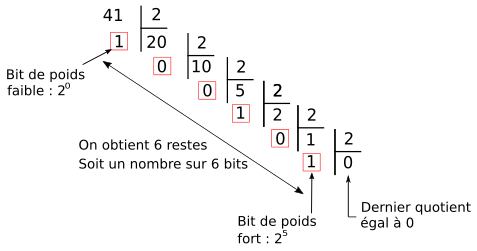
\includegraphics{img/div-succ-binaire.png}
\caption{div-succ-binaire.png}
\end{figure}

Comme pour la méthode précédente, on obtient \(41_{10}=101001_{2}\)

Le nombre obtenu est sur 6 bits mais sur 1 octet : \(00101001\)

    \hypertarget{exercice}{%
\subsection{Exercice}\label{exercice}}

Donner l'écriture décimale des nombres entiers positifs codés en binaire
sur 1 octet.

\begin{enumerate}
\def\labelenumi{\arabic{enumi}.}
\tightlist
\item
  \(01010101\)
\item
  \(10101010\)
\item
  \(10111010\)
\item
  \(11001101\)
\end{enumerate}

\hypertarget{exercice-1}{%
\subsection{Exercice}\label{exercice-1}}

Donner l'écriture binaire des nombres entiers positfs exprimés en
décimal. Faire apparaître le calcul.

\begin{enumerate}
\def\labelenumi{\arabic{enumi}.}
\tightlist
\item
  \(13\)
\item
  \(54\)
\item
  \(132\)
\item
  \(245\)
\end{enumerate}

    \hypertarget{numuxe9ration-hexaduxe9cimale}{%
\section{Numération hexadécimale}\label{numuxe9ration-hexaduxe9cimale}}

\hypertarget{duxe9finition}{%
\subsubsection*{Définition}\label{duxe9finition}}

La numération \textbf{hexadécimale} est une numération en \textbf{base}
\(16\).

Cette numération utilise donc \(16\) chiffres : - Les 10 chiffres de la
numération décimale : de \(0\) à \(9\); - et on ajoute les 6 premières
lettres de l'alphabet : A, B, C, D, E et F.

En notation décimale : \(A=10\), \(B=11\), \(C=12\), \(D=13\), \(E=14\)
et \(F=15\).

En notation binaire sur 4 bits : \(A=1010\), \(B=1011\), \(C=1100\),
\(D=1101\), \(E=1110\) et \(F=1111\).

\hypertarget{exemple}{%
\subsubsection*{Exemple}\label{exemple}}

Soit les nombres entiers \(41\) et \(206\) en notation décimale.

En notation hexadécimale : \begin{align*}
41_{10} &= 2 \times 16^{1} + 9 \times 16^{0} \text{  donc  } 41_{10} = 29_{16}\\
206_{10} &= 12 \times 16^{1} + 14 \times 16^{0} \text{  donc  } 206_{10} = CE_{16}
\end{align*}

    \hypertarget{conversion-duxe9cimale-en-hexaduxe9cimale}{%
\subsection{Conversion décimale en
hexadécimale}\label{conversion-duxe9cimale-en-hexaduxe9cimale}}

\hypertarget{muxe9thode}{%
\subsubsection*{Méthode}\label{muxe9thode}}

La conversion d'un nombre décimal en hexadécimal est délicate. On peut
utiliser les mêmes méthodes que pour la conversion en binaire, à savoir
par soustraction de puissances de \(16\) ou les divisions euclidiennes
par \(16\).

\hypertarget{exemple}{%
\subsubsection*{Exemple}\label{exemple}}

Soit le nombre entier positif \(453\) à convertir en hexadécimal:
\(453_{10}=1\)C\(5_{16}\)

\begin{figure}
\centering
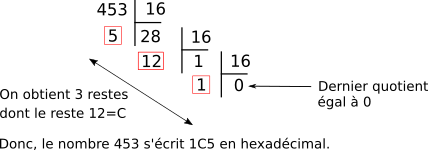
\includegraphics{img/div-succ-hexa.png}
\caption{div-succ-hexa.png}
\end{figure}

\hypertarget{conversion-binaire-en-hexaduxe9cimale}{%
\subsection{Conversion binaire en
hexadécimale}\label{conversion-binaire-en-hexaduxe9cimale}}

\hypertarget{remarque}{%
\subsubsection*{Remarque}\label{remarque}}

La conversion de binaire à hexadécimal et inversement est beaucoup plus
simple.

Chaque chiffre hexadecimal correspond à un groupe de 4 bits appelé
\textbf{quartet}.

\hypertarget{muxe9thode-1}{%
\subsubsection*{Méthode}\label{muxe9thode-1}}

Lorsqu'une valeur binaire est codée sur un octet, on casse en 2 fois 4
bits le nombre pour obtenir 2 quartets.

Chaque quartet correspond à un chifre hexadécimal.

\hypertarget{exemple-1}{%
\subsubsection*{Exemple}\label{exemple-1}}

Le nombre \(41\) s'écrit \(00101001\) en binaire soit
\(\underbrace{0010}\underbrace{1001}\).

On obtient les quartets \(0010\) et \(1001\).

Le premier quartet vaut \(2\) et le second quartet vaut \(9\) en
hexadécimal.

Donc: \[41_{10}=00101001_{2}=29_{16}\]

    \hypertarget{exercice}{%
\subsection{Exercice}\label{exercice}}

Convertir en notation binaire et décimale les nombres suivants écrits en
notation hexadécimale:

\begin{enumerate}
\def\labelenumi{\arabic{enumi}.}
\tightlist
\item
  3E
\item
  4F8B
\item
  AA553C
\end{enumerate}

\hypertarget{exercice-1}{%
\subsection{Exercice}\label{exercice-1}}

Convertir en écriture hexadécimale les nombres suivants (attention à la
base):

\begin{enumerate}
\def\labelenumi{\arabic{enumi}.}
\tightlist
\item
  \(168_{10}\)
\item
  \(1001_{10}\)
\item
  \(10100101_{2}\)
\end{enumerate}

    \hypertarget{pour-info}{%
\section{Pour info}\label{pour-info}}

Il existe d'autres bases de numération comme la base octale. Sur les
systèmes d'exploitation Linux, les droits des utilisateurs sont exprimés
en base octale. Un utilisateur qui a les droits 777 sur un dossier ou un
fichier a tous les droits.

De façon générale, une base de valeur \(b\) permet d'écrire des nombres
dans cette base s'exprimant par :
\[a_{n} \times b^{n} + a_{n-1} \times b^{n-1} + \ldots + a_{1} \times b^{1} + a_{0}\]
Les coefficients \(a_{i}\) sont strictement inférieurs à \(b\).

\hypertarget{exemple}{%
\subsubsection*{Exemple}\label{exemple}}

En base octale \(b=8\), les coefficients sont les nombres entiers
compris entre \(0\) et \(7\).

Le nombre \(755\) a pour valeur :
\(7 \times 8^{2}+5 \times 8^{1} + 5 = 493\) en base 10.

    
    
    
\end{document}
